
%: ----------------------- introduction file header -----------------------
\chapter{Introduction}

%\begin{flushright}
%I am just now beginning to discover the difficulty 
%\linebreak
%of expressing one's ideas on paper. As long as it 
%\linebreak
%consists solely of description it is pretty easy, but  
%\linebreak
%where reasoning comes into play, to make a proper
%\linebreak
%connection, a clearness \& a moderate fluency, is to me,   
%\linebreak
%as i have said, a difficulty of which i had no idea.
%\linebreak
%C. Darwin
%\end{flushright}
\ifpdf
    \graphicspath{{1_introduction/figures/PNG/}{1_introduction/figures/PDF/}{1_introduction/figures/}}
\else
    \graphicspath{{1_introduction/figures/EPS/}{1_introduction/figures/}}
\fi

This PhD thesis aims at proposing, developing and validating new Evolutionary Algorithm (EA) variants for solving design-optimization problems tools with reasonable computing cost. This is extremely useful when handling large-scale industrial optimization problems, such as in the fields of thermal and hydraulic turbomachines. The developed EA variants, enhanced with the proposed add-on features, should be able to produce high quality designs, at acceptable, according to the industrial standards, turn-around time. The later is, in fact, necessary for EAs to become a design-optimization tool routinely used in an industrial environment. To reduce the optimization turn-around time, a method which overcomes the standard shape parameterization techniques which, in real-world applications, introduce a great number of design variables, is firstly proposed. Instead, this thesis proposes and evaluates a way to use the information residing into a small number of archived designs, made available from similar successful projects worked out in the past. The proposed method requires the solution of problems with much less design variables which can be carried out by EAs at reasonable computing cost. The proposed method combines ``ideas'' from the theory of Knowledge Based Systems (KBS) with the  EAs, giving rise to a fast design method that will be referred to as Knowledge Based Design (KBD). Furthermore, the degradation in EAs efficiency/speed when used to solve ill-posed problems motivated the development of a method capable of recovering a great part of the efficiency loss. This method makes use of the Principal Component Analysis (PCA) to identify the directions in the design space that, if used to define new design variables, would result in a well-posed optimization problem.  This information is, then, used to modify the evolution operators so as to operate in the most well-posed problem possible and therefore recover as much efficiency loss as possible.  A by-product of the aforementioned method was the assignment of ``importance'' to each and every design variable (or design space coordinate). Metamodel-assisted EAs (MAEAs), in which the costly problem-specific evaluation tool (CFD code, in the applications this thesis is concerned with) is replaced by surrogate evaluation models or metamodels (usually trained artificial neural networks, ANNs, polynomial regression methods, etc.) may benefit from the importance-based ranking of the design space coordinates, in order to overcome problems caused by the so called curse of dimensionality. A method that utilises this, via appropriate truncation of the ANN entries, in order to create metamodels that are able to better drive the evolution is proposed in this thesis.  

All of the aforementioned methods are validated in cases ranging from  some low-cost mathematical optimization benchmarks to 2D compressor cascade designs and, finally, to the design of industrial 3D hydraulic turbines and a 3D compressor cascade with tip clearance installed at LTT/NTUA. The mathematical benchmarks have low computing cost and allow, thus, the exhaustive investigation of methods by performing several runs, using different seeds for the random number generator, on the same case. The presented 2D cases allow the demonstration of the methods in simple aerodynamic optimization cases. Furthermore, two types of hydraulic turbines, a Francis and a new type named Hydromatrix$\circledR$, are used to validate the performance of the aforementioned methods in large-scale industrial applications. A number of performance metrics are introduced and, depending on the case, are combined to form the objectives and constraints. The Hydraulic turbomachinery design cases consider more than one operating points, leading to an increased cost per CFD-based evaluation, which makes even more valuable the reduction in the number of evaluations required to reach the optimal solution(s).  Finally, the airfoil of the 3D compressor cascade installed at LTT/NTUA, aiming at minimum total pressure losses, is optimized.     


This PhD thesis is based on EAs developed in a number of previous PhDs \cite{phd_Giotis,phd_Karakasis,phd_Kampolis,phd_Vera} performed at the Parallel Cfd and Optimization unit of LTT/NTUA (PCOpt/NTUA). The previous PhD theses created the algorithmic basis (platform),  which the newly proposed methods were built upon. This EA-based platform, referred to as the EASY (Evolutionary Algorithm SYstem \cite{EASYsite}) includes, the basic EA, optionally enhanced by parallel search (PEA), incorporation of ANNs as metamodels (MAEA) and hierarchical optimization schemes (HEA) provided fertile ground for the new methods proposed by this PhD thesis.                       
 
%An overview of the use of optimization methods for fluid dynamic problems, a review on the previews works by PCOpt this thesis has build upon and the thesis structure follow.

\section{CFD-based Optimization}

An overview of CFD-based optimization methods is presented in this section. CFD-based optimization methods enjoy grate interest (figure \ref{pubs.CFD}) from both academia and industry since the performance, and therefore the price, of products ranging from cars and aircrafts to thermal and hydraulic turbomachines  depends heavily on their aero/hydrodynamic performance. The first ever essay that dealt with the subject was done in $1910$ by Hadamard \cite{Had10} and utilised variation theory for partial differential equations governing problems.   

\begin{figure}[h!]
\begin{minipage}[b]{1\linewidth}
 \centering
 \resizebox*{!}{8 cm}{\includegraphics{OptimizationCFD.eps}}
\end{minipage}
\caption{Number of publications regarding CFD-based optimization on science direct.} 
\label{pubs.CFD}
\end{figure}

In order to scope the interest of the scientific community on the subject an inexact internet-based literature search has been carried out using the scientific literature search tool ``Science direct'' (http://www.sciencedirect.com/). The search criterion was (Optimization $AND$ CFD) $OR$ (Optimization $AND$ Computational Fluid Dynamics).  This is obviously a non-specific search, it is nevertheless capable to identify the trend associated with CFD-based optimization.  The steadily growing number of publications in the last five years, as seen in figure \ref{pubs.CFD}, reveals the growing interest in the subject in hand. Therefore, the upgrades proposed by this thesis are of interest to a, great and increasing in number, community of scientist not only restricted in the field of turbomachines.     
 
A prerequisite for any CFD-based optimization is the availability of a fast and reliable way to evaluate each candidate solution. This is achieved through the use of Computational Fluid Dynamic (CFD) (hence the term CFD-based optimization) methods that numerically solve the differential equations governing the fluid motion. Nowadays, the relatively cheap access to powerful computational means has transformed CFD into a reliable and fast evaluation tool and, therefore, the optimization methods that utilize it are flourishing. The strong correlation among CFD-based optimization and computational resources is greatly enhanced in cases where a number of disciplines, ranging from structural analysis to manufacturing and economics, are used to evaluate the candidate solutions (multidisciplinary optimization). The fact that the fluid dynamic, structural and economical objectives may be contradictory adds extra difficulty to the optimization procedure.           
 
Also, important part of the optimization procedure is the definition of the design variables. The aim of an optimization algorithm is to locate the set of design variables that minimize the user defined cost function(s).  In CFD-based optimization, the objectives are defined so as to describe the quality of the design. Typical objectives are; the maximization of efficiency, the minimization of the deviation from given target distributions for the velocity or the pressure, the minimization of total pressure losses or cavitation index (in hydraulic turbomachines), etc.  Design-optimization problems with more than one objectives (multi-objective optimization, MOO) can be solved simply by concatenating the objectives into a single one through the use of weights. The difficulty of choosing appropriate weight values and the failure of the approach in non-convex optimization problems are two of its main weaknesses.  An improved way to solve MOO problems is the use of dominance based methods that rank the candidate solutions accoutring to Pareto dominance. This method returns a set of optimal solutions namely the so-called set of non-dominated solutions or Pareto front, where none of them  is dominated by any other regarding all the objectives.  Therefore, the choice of the optimal solution to be adopted relies on other criteria to be used by the decision maker.  The design-optimization problem can, also, be subject to a number of constraints. In CFD-based optimization, typical constraints are related to geometrical quantities (usually, thickness constraints), structural quantities such as maximum stress or deflection and flow-related quantities such as the minimum flow turning or the cavitation index.          

In general, CFD-based optimization can be classified in two categories, the direct and inverse design-optimization methods. Direct methods solve the optimization problem after a number of trials \cite{phd_Giotis,phd_Kampolis,phd:papadim,kn:Emm2002,kn:Emm2004}. Each trial involves the geometry generation, CFD predictions, the objective function estimation and ,likely, its gradient computation.  On the contrary, inverse design-optimization methods (should not be confused with inverse design problem \footnote{Inverse design problems use as cost function the deviation from a desirable state.} that can be solved by direct methods) \cite{chav:95,ded:95} begin from a set of desirable flow field characteristics (i.e. boundary layer) and solve the inverse problem to define the geometry. The major advantage of inverse methods is their speed and their ability to begin without a initial geometry. Their most noticeable drawback, on the other hand, is their inability to handle constrained optimization problems. The inverse methods developed by LTT/NTUA are based on the Le Foll method \cite{lefoll} which uses two parameters to control the incompressible (laminar and turbulent) boundary layer. This method was extended to facilitate compressibility \cite{pap69}, surface curvature effects in the calculation of the turbulent boundary layer \cite{pap70} and boundary layer separation \cite{pap81} and was later used for the design of both axial and radial turbomachines. Based on the above classification, this PhD thesis is dealing with direct design-optimization methods.  

Examining the characteristics of the design-optimization method itself,  they are classified into deterministic and stochastic. Deterministic design-optimization methods were used first in CFD-based optimization mainly due to their solid mathematical background and fast convergence, locate the optimal solution with less candidate solution trials. The weakness of deterministic optimization methods is the necessity to calculate the gradient of the objective function(s) with respect to the design variables. This limits the choice of objective functions since they must be differentiable. Furthermore, the cost of the gradient calculation can be noticeably high if access to the evaluation software source code is not granted and therefore adjoin method cannot be used thus finite differences are utilised. Furthermore, their difficulty in solving MOO problems by computing the ensemble of non-dominated solutions and the danger risk of being trapped into local minima (being gradient based methods) have to mentioned.        

For deterministic optimization methods, used in fluid dynamics design problems, except of the search method (steepest decent, Newton, e.t.c.) the most important part is the gradient calculation. The use of finite differences, as mentioned above, is not suitable since it requires, at least, as many flow predictions as the design variables. The use of adjoint techniques, though, can reduce this number to a single flow field prediction irrespective of the number of design variables. Due to the need of significant time and effort investment required by the engineer (in the form of mathematical preparation and additional programming), adjoint techniques were not used in CFD-based optimization since the mid $80^s$ \cite{piron:84, kn:Jame88, kn:Jame94, kn:Jame95}.  The two variants of adjoint techniques differ in the way that the discretized adjoit equations are formed. The continuous adjoint variant \cite{kn:Jame94, kn:Ander99,phd:papadim}, is based on the continuous form of the flow equations in order to derive the adjoint ones. On the other hand, in the discrete adjoint variant the adjoint equations result directly from the discretized flow equations \cite{kn:Elliott96, anderson:99}. The main disadvantage of the discrete adjoint variant against the continuous one, is the increased memory requirements. The accuracy of the two adjoint formulations is, theoretically, identical; in practice this is true only for very dense grids.  A more detailed presentation of adjoint methods used for fluid dynamic optimization can be found in \cite{phd:papadim}.        

Stochastic optimization methods, on the other hand, do not suffer for the risk of getting trapped into local minima due to the probabilistic nature of the candidate solution generation procedure. Furthermore, the differentiability of the objective is not required. An additional positive feature of stochastic optimization methods, especially regarding industrial use, is their ability to accommodate any problem merely by providing the evaluation software, without necessary having access to its source code. Their main drawback, though, is the need to evaluate a great number of candidate solutions before reaching the optimum. Thus, significantly increasing the overall computational cost of the optimization procedure. This PhD is dealing with  stochastic optimization methods and more precisely with EAs. 

The use of EAs in CFD-based optimization was delayed up until the mid $90^s$ mainly due to their, as mentioned above, big computational cost. The first essays on the subject \cite{kn:Quag95,per:95,kn:Gala96} present automated EA-based design-optimization procedures for aerodynamic design-optimization problems. Soon after came the first attempts to reduce the cost of the overall optimization procedure, mainly by adapting the available coding and evolution operators. This trend continued with the hybridization with deterministic optimization methods. For instance, in \cite{kn:Mar97} and \cite{kn:Fost97}, an EA is used to spot the starting point for a deterministic optimization method. Later, in \cite{dennis:99}, EAs were hybridized with Sequential Quadratic Programming (SQP) for constrained shape optimization problems. Furthermore,  the use of distributed EAs \cite{kn:Door1997,kn:SefrThes}, surrogate evaluation models \cite{kn:Ratl98,kn:Gio99,kn:Gian1999,kn:EBNK,phd_Kampolis}, hierarchical schemes \cite{kn:Eby1998,kn:Sef2000,knowles00mpaes_x41,desideri03,phd_Kampolis} and concurrent evaluations in a multiprocessor environment  \cite{kn:LeeH96,phd_Giotis,phd_Vera} were proposed. Nowadays, the appeal of CFD-based EAs optimization regarding industrial-scale real-life engineering problems is increasing, mainly due to the  computational resources availability and the potential for significant gains both in design quality and design time and, therefore, cost.  This PhD thesis is dealing with the use of EAs for solving industrial scale design-optimization problems in the fields of thermal and hydraulic turbomachines in acceptable for industry turn-around time.   


\begin{figure}[h!]
\begin{minipage}[b]{1\linewidth}
 \centering
 \resizebox*{!}{8 cm}{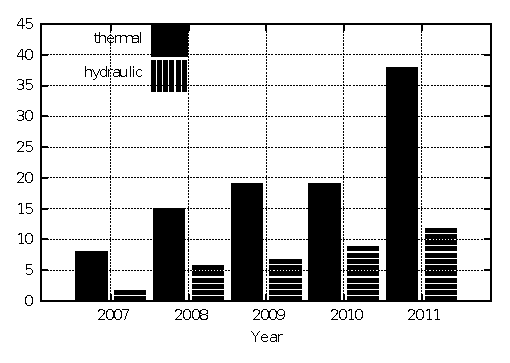
\includegraphics{hydrtherm_m.eps}}
\end{minipage}
\caption{Number of publications regarding optimization in thermal and hydraulic turbomachines on science direct.} 
\label{pubs.turbo}
\end{figure}
 

Regarding CFD-based optimization in the fields of thermal and hydraulic turbomachines a inexact internet-based literature search has been carried out as before. The search criterion where; (a) optimization $AND$ thermal $AND$ turbomachines and (b) optimization $AND$ hydraulic $AND$ turbomachines. Though  this is  a non-specific search it reveals the steadily growing number of publications, in both thermal and hydraulic turbomachiens, over the last five years, as seen in figure \ref{pubs.turbo}. These by it self reveals the growing interest of the scientific community for CFD-based optimization in both fields. 

In ASME 2011 Turbo Expo conference $24$ papers were published regarding EA-based optimization in the field of thermal turbomachines, either CFD-based or not. Most of them are handling a low number of design variables, $N$ up to $15$, and only three \cite{Georg2011,Marcel2011,Kevin2011} are handling high dimensional problems $N\!>\!30$. In \cite{Georg2011} the application of an axisymmetric endwall contour for compressors is investigated and a EA-based optimization of the outer casing and the corresponding blade tip airfoil section of a typical gas turbine high pressure compressor stage with a high number of design variables ($N\!=\!38$) is presented. In \cite{Marcel2011} the high-dimensional ($N\!=\!210$) constrained multiobjective optimization of a fan stage  using EAs enhanced by metamodels is presented. In \cite{Kevin2011} an EA-based axisymmetric multi-disciplinary optimization approach for compressors is presented and applied to the design of a three stage booster with $N\!=\!53$ design variables. The aforementioned papers even though they have high number of design variables they typically start from an almost optimal design and therefore are able to assign significantly low range to their design variables, i.e. \cite{Marcel2011} starts from a ``pre-optimized'' design and \cite{Georg2011} has variable's range in the tip clearance magnitude. The first method (KBD) proposed by this thesis is dealing with both high-dimentional ($N\!>\!300$), high-variable' range optimization problems.      

In IAHR 2010 conference $5$ paper regarding optimization in the field of hydraulic turbomachines were published, among them $3$ \cite{Raimunda2010,Kyriacou2010,Popa2010} used EAs. In \cite{Popa2010} the weekly operation of a multipurpose
hydroelectric development, including a pumped storage plant was optimized by an EA. In \cite{Raimunda2010} a $N\!=\!2$ optimization problem concerning the design of an axial compressor cascade using a metamodel assisted EA was presented.  In \cite{Kyriacou2010} a $N\!=\!336$ optimization problem concerning the design of a Francis hydraulic turbine was presented, the later was a result of this PhD thesis. 


Significant work, regarding CFD-based optimization in the fields of thermal and hydraulic turbomachines has been made in NTUA by the Laboratory of Thermal Turbomachines (LTT) and Laboratory of Hydraulic Machines (LHM) respectively. 
Concerning thermal turbomachines, a number of papers regarding both deterministic and stochastic optimization methods have been published. These were related to the optimal design of components of thermal turbomachines, such as compressor cascades, using a variety of optimization techniques.  An indicative subset of them is mentioned below. The use of stochastic optimization methods coupled with computational intelligence is presented in \cite{LTT_2_018,LTT_2_020,LTT_2_023}. There, the use of artificial neural networks as metamodels, in order to assist the EA when dealing with costly evaluation tools such as CFD codes, were proposed, in fact these techniques are in use throughout this PhD thesis. In \cite{LTT_2_026}, the use of metamodels trained both on responses and gradients is proposed and used in the inverse design of a 3D peripheral cascade. In \cite{LTT_2_031} the hierarchical distributed metamodel-assisted evolutionary algorithm was used for the loss minimization of a compressor cascade. In \cite{LTT_2_040} an asynchronous evolutionary algorithm is used for the optimal design of a 2D compressor cascade and in \cite{LTT_2_045} a grid-enabled asynchronous metamodel-assisted evolutionary algorithm was utilized for the optimization of a 3D annular compressor cascade. Furthermore, in \cite{LTT_2_032}, a adjoint-based  deterministic optimization method is proposed for the total pressure losses minimization in turbomachinery cascade.  In \cite{LTT_2_049}  the computation of the exact Hessian matrix for efficient optimization using the Newton equation for the total pressure losses minimization in turbomachinery cascade is proposed. Multilevel strategies that combine adjoint based methods with metamodels assisted evolutionary algorithms for turbomachines were proposed in \cite{LTT_3_092}.


Concerning CFD-based optimization in the field of hydraulic turbomachines, the work done by LHM is related to; a) the optimal design of components of hydraulic machines, such as runner blades, and b) the optimal design of complete hydroelectric power plants and energy storage plants in combination with other forms of renewable energy generation sources, such as wind energy. An indicative subset of these work can be fount in the publications listed below. In \cite{Anagno2} an EA was used to improve the design of a microchannel structure used in a valveless micropump, the so-called ``Tesla-Type Valve''. In \cite{Anagno4} the fast Lagrangian approach was used in collaboration with a EA to design an optimal Turgo turbine. The optimal sizing of a run-of-river small hydroelectric power plant utilizing an EA was proposed in \cite{Anagno3}. Furthermore, in \cite{Anagno5,Anagno6} the optimization of pumped-storage for wind power plants is presented.

   

\section{Previous work by LTT/NTUA} % section headings are printed smaller than chapter names
\label{PRW}
An overview of four previous PhD theses on EAs carried out at the same research group of NTUA is due. 

Giotis, \cite{phd_Giotis}, developed a generalised EA able to combine components of the two most widely used evolutionary optimization methods, namely Genetic Algorithms (GAs) and Evolutionary Strategies (ESs). Furthermore, in the same thesis, the use of artificial neural networks as local metamodels, trained on previously evaluated candidate solutions was proposed in order to reduce the computational burden. To reduce the wall clock time of the optimization, parallel processing via the PVM protocol was also introduced. 

Karakasis, \cite{phd_Karakasis}, further improved the EA efficiency by focusing on the optimal use of metamodels in multi objective optimization problems. The main achievement of \cite{phd_Karakasis} was that the MAEA became equally efficient in both multi- and single- objective problems by overcoming problems related to; (a) the fact that the previously computed individuals, by the EA, in a multi-objective optimization problem are spread rather than clustered around the sought optimal solution and (b) the presence of outliers that require special treatment. Distributed EAs (DEAs), were programmed and validated, these aimed at increasing the parallel efficiency of EAs, improving convergence and avoiding premature population stagnation. Furthermore the notion of Hierarchical EAs (HEAs) was introduced for the first time which was later refined in \cite{phd_Kampolis}.    In \cite{phd_Karakasis}, the use of a DEA at each level of the HEA associated with different evaluation models was proposed.

In Kampolis, \cite{phd_Kampolis}, the HEAs were refined by introducing apart from hierarchy regarding the evaluation tool, hierarchical variants with respect to the parameterization and, even, the search method thus making possible the combination of EAs with deterministic optimization methods combining the advantages of both, stochastic and deterministic, classes. Furthermore, the introduction of gradient trained artificial neural networks was proposed during the same thesis.          

Part of the fourth PhD thesis, Asouti in \cite{phd_Vera}, aimed at increasing the parallel efficiency of EAs or MAEAs. This was achieved by the introduction of the so-called Asynchronous EA (AEAs) or Asynchronous MAEAs (AMAEAs). By utilizing a number of strongly interconnected demes, the asynchronous variants may circumvent the "end of generation" synchronization barrier and, thus, non interruptibly use all the available processors.    

\section{Structure of this Thesis} % section headings are printed smaller than chapter names
A short overview of the chapters of this PhD thesis follows:

Chapter $2$ presents the, pre-existing, algorithmic basis of this PhD. This includes the generalized EA with all its evolution operators, the metamodel assisted EA and the Hierarchical EA.

Chapter $3$ is concerned with the first innovative method proposed in this PhD thesis, i.e. the one which was previously referred to as the Knowledge Based Design (KBD) method. In this chapter, a short overview of knowledge based systems and, especially the case based reasoning (CBR) is presented. Then the proposed KBD method is presented in detail and used to perform the design of a 2D compressor cascade, in order to demonstrate the merits of the proposed method.

Chapter $4$ deals EAs and MAEAs suitable to solve ill-posed optimization problems. First the presentation of the characteristics of an ill-posed optimization problem takes place. Then the degradation of EA efficiency when they are used to solve ill-posed optimization problems is investigated. Furthermore an innovative way to estimate directions in the design space that, if used as design variables, would result in a well-posed problem is proposed.  New evolution operators, the so-called PCA-driven evolution operators are proposed, in order to recover the aforementioned EA efficiency loss and then are  validated. Furthermore the use of the importance information, resulting form the PCA is used to enhance metamodel efficiency. Finally the combined gain of the aforementioned proposed methods is validated through a 2D compressor cascade design-optimization case.

In chapter $5$, the efficiency gains from the use of the methods proposed in this thesis are used to solve large-scale industrial cases from the field of hydraulic turbomachines. In more detail, the parameterization, grid generation and CFD tools in use, are presented. Quality metrics that demonstrate each hydraulic turbine quality regarding cavitation, blade loading and draft-tube coupling are introduced. Then the optimization of a Francis turbine, in the scope of a modernization/rehabilitation project, is used to demonstrate the merits of the KBD method as opposed to a conventional EA. Furthermore the optimization of a new type of hydraulic turbine, namely the Hydromatrix$\circledR$, is used to demonstrate the merits of the proposed PCA-driven evolution operators.

Chapter $6$ is dedicated to the design-optimization of the compressor cascade installed at LTT/NTUA. This case is used to investigate the combined effects of the use of PCA-driven evolution operators combined the PCA-assisted metamodels as proposed in Chapter $4$.

Finally Chapter $7$ presents the conclusions of this PhD thesis.      

%: ----------------------- HELP: references
% References can be links to figures, tables, sections, or references.
% For figures, tables, and text you define the target of the link with \label{XYZ}. Then you call cross-link with the command \ref{XYZ}, as above
% Citations are bound in a very similar way with \cite{XYZ}. You store your references in a BibTex file with a programme like BibDesk.


%%%%%%%% template for figures
%see fig \ref{A common glucose polymers}
%\figuremacro{EAvsPCA_zdt3}{A common glucose polymers}{The figure shows starch granules in potato cells, %taken from \href{http://molecularexpressions.com/micro/gallery/burgersnfries/burgersnfries4.html}{Molecular %Expressions}.}

%%: ----------------------- HELP: adding figures with macros
%% This template provides a very convenient way to add figures with minimal code.
%% \figuremacro{1}{2}{3}{4} calls up a series of commands formating your image.
%% 1 = name of the file without extension; PNG, JPEG is ok; GIF doesn't work
%% 2 = title of the figure AND the name of the label for cross-linking
%% 3 = caption text for the figure

%%: ----------------------- HELP: www links
%% You can also see above how, www links are placed
%% \href{http://www.something.net}{link text}

%\figuremacroW{EAvsPCA_zdt3}{Title}{Caption}{0.8}
%% variation of the above macro with a width setting
%% \figuremacroW{1}{2}{3}{4}
%% 1-3 as above
%% There you go. You already know the most important things.



